\documentclass[a4j,titlepage]{jarticle}
\usepackage[dvipdfmx]{graphicx}
\usepackage{ascmac}
\usepackage{float}
\usepackage{amssymb}%にやりイコールを使う
\usepackage{multirow}
\usepackage{multicol}
%\usepackage{color}

\begin{document}

\title{2022 年度 3 回生前期学生実験 HW  \\ \bf team02 実施状況報告書}
% ↓ここに自分の氏名を記入
\author{実施状況報告書作成者:植田健斗\\
グループメンバー:\\伊藤舜一郎 (学籍番号:1029-32-7548)
\\植田健斗 (学籍番号:1029-32-6498)}
\西暦
\date{提出期限:5月12日18時 提出日: \today} % コンパイル時の日付が自動で挿入される
\maketitle
\newpage

\section{モジュール分割}

それぞれの機能を持った回路ごとにモジュール分割した。
各回路につけた名前は図\ref{moduleSplit0422}に示した通りである。(次の章の図\ref{rolesDivision0422}でまとめてある。)
赤色の図形で囲まれた箇所がモジュールになっており、各モジュールの名前は赤色で書いてある。外部入力は16bitの入力ピンをあらわしている。赤色で囲われていない長方形は外部入力を除いてレジスタをあらわしている。太線はマルチプレクサを表し、その近くに書かれた文字は制御部から各マルチプレクサに送る制御信号の名前をあらわしている。マルチプレクサの近くに書かれた0と1の数字は制御信号がその値になったときにつながるデータパスを表している。


\begin{figure}[H]
    \begin{center}
    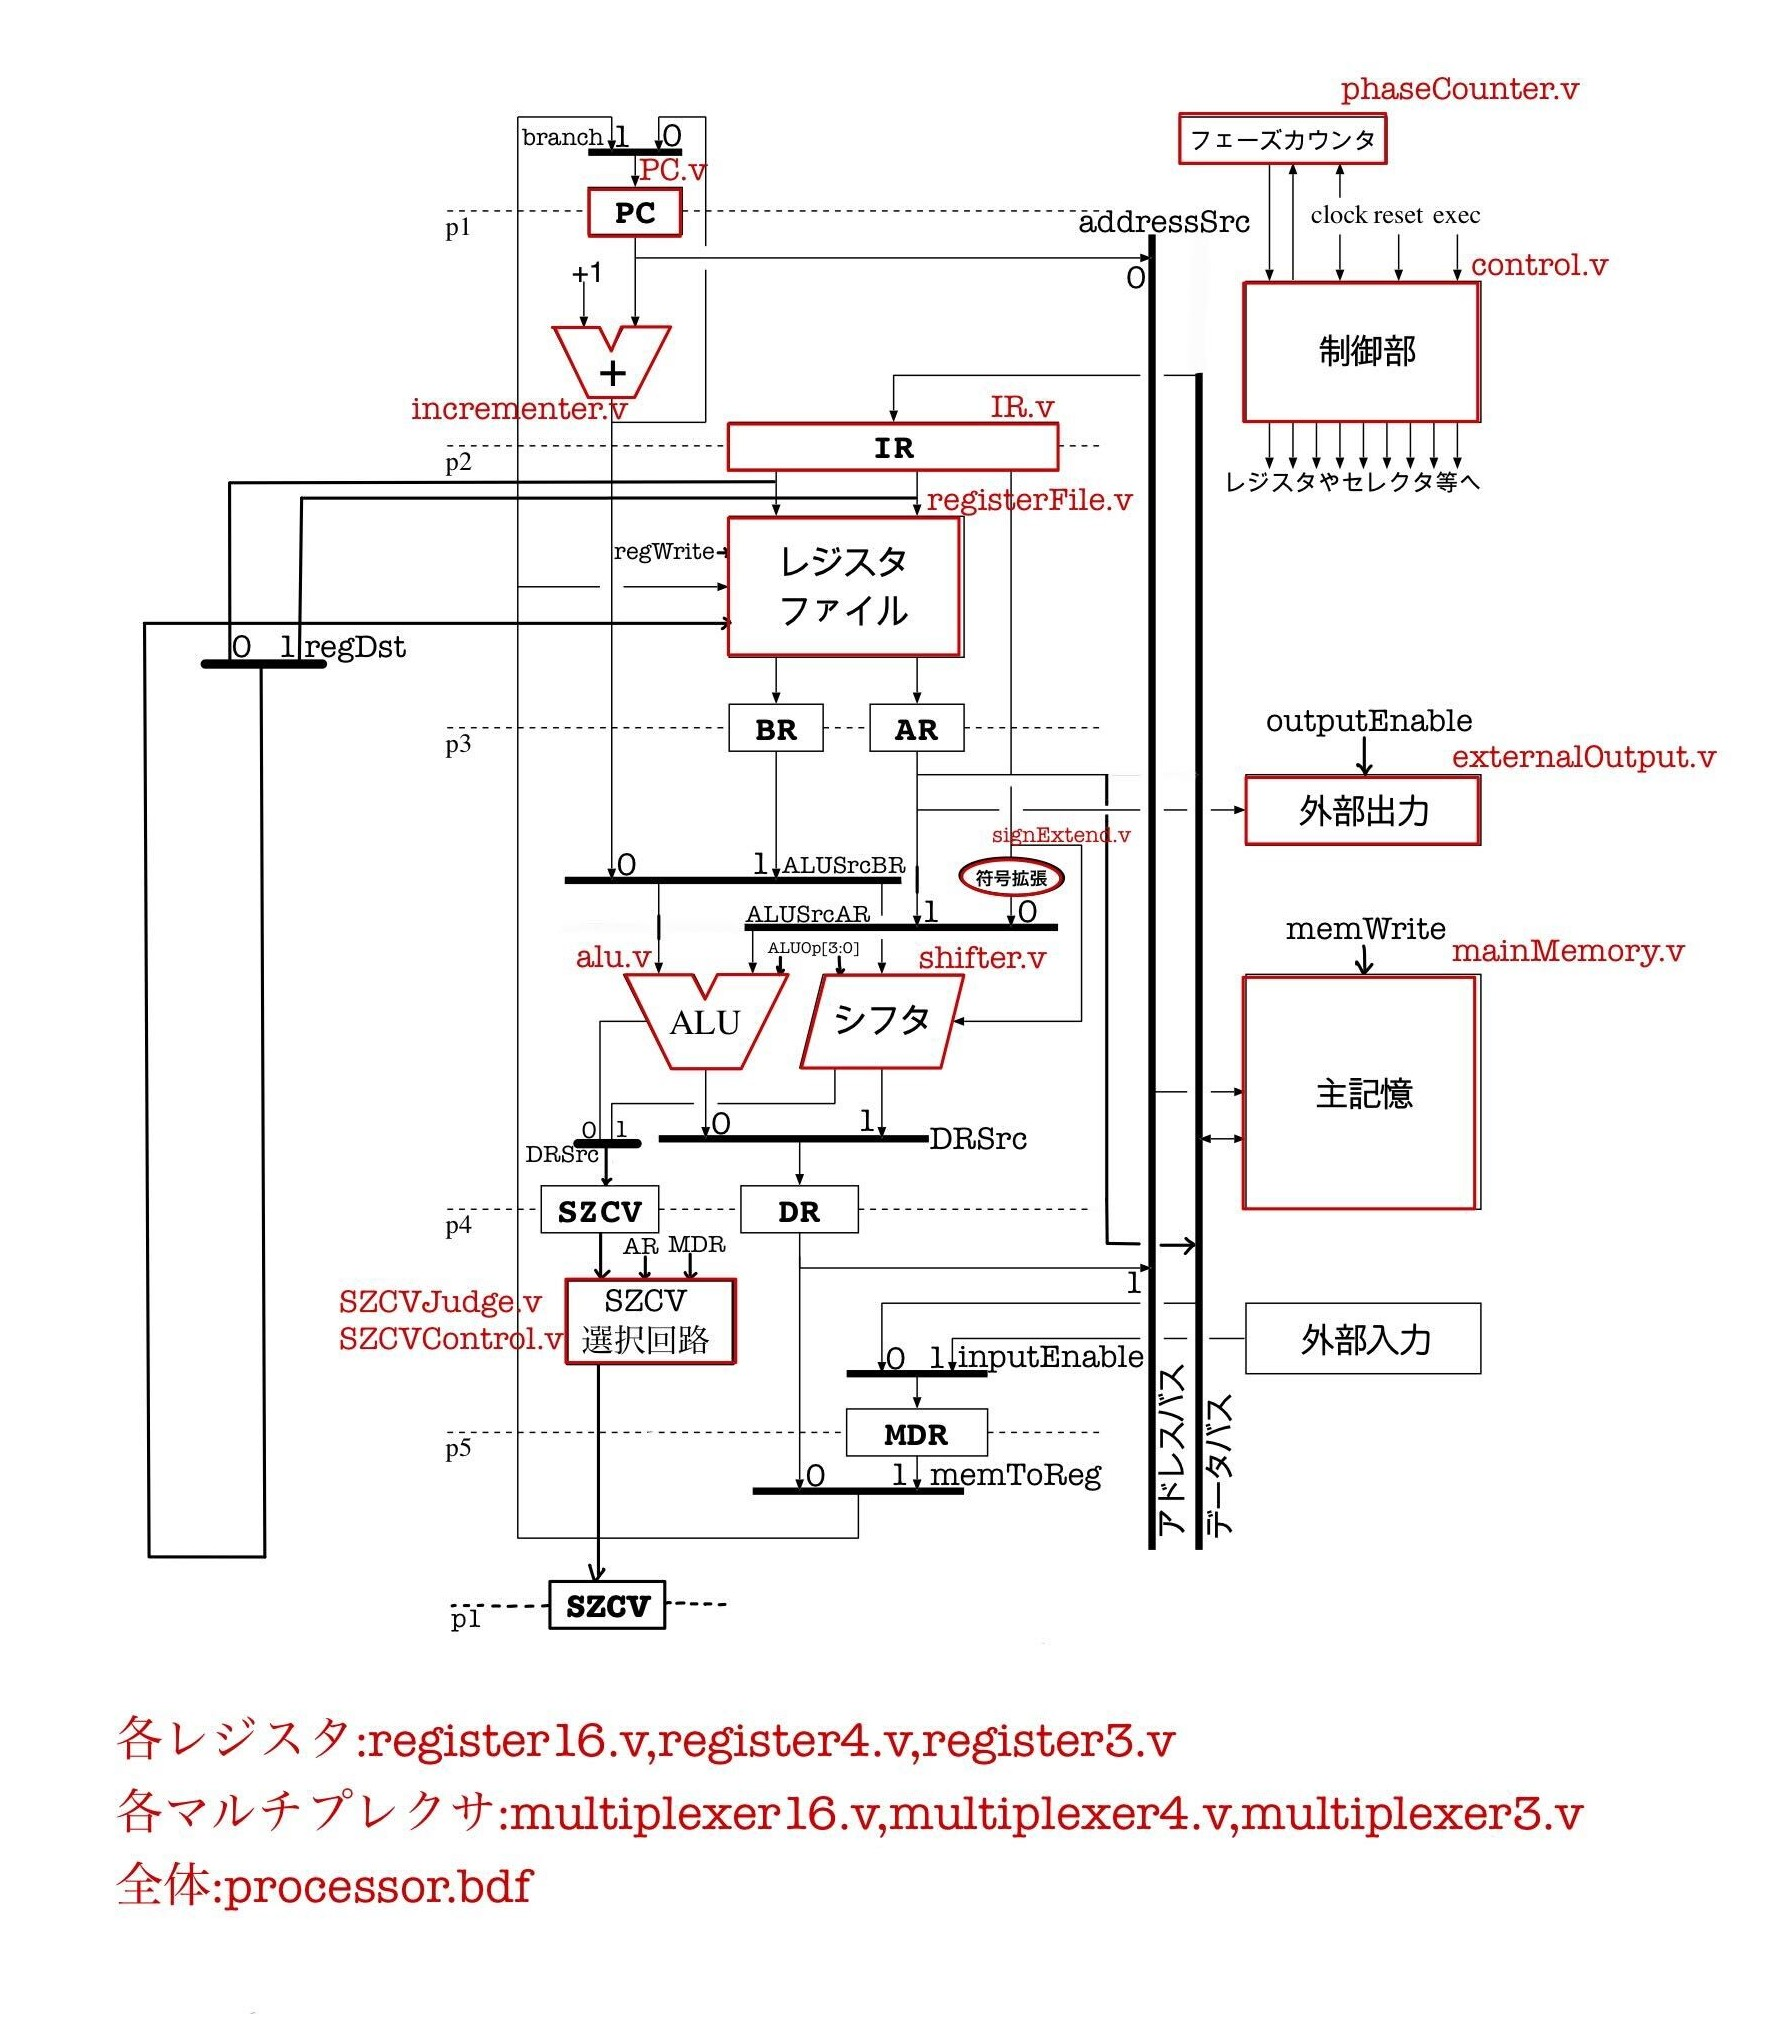
\includegraphics[scale = 0.22]{moduleSplit0506.jpg}
    \end{center}
    \caption{モジュール分割}
    \label{moduleSplit0422}
\end{figure}

\section{役割分担}

役割分担の表を以下の図\ref{rolesDivision0422}に示す。拡張機能はまだ具体的に構成が決まっていないので、現在作成した回路の役割分担のみ記してある。




\begin{figure}[H]
    \begin{center}
        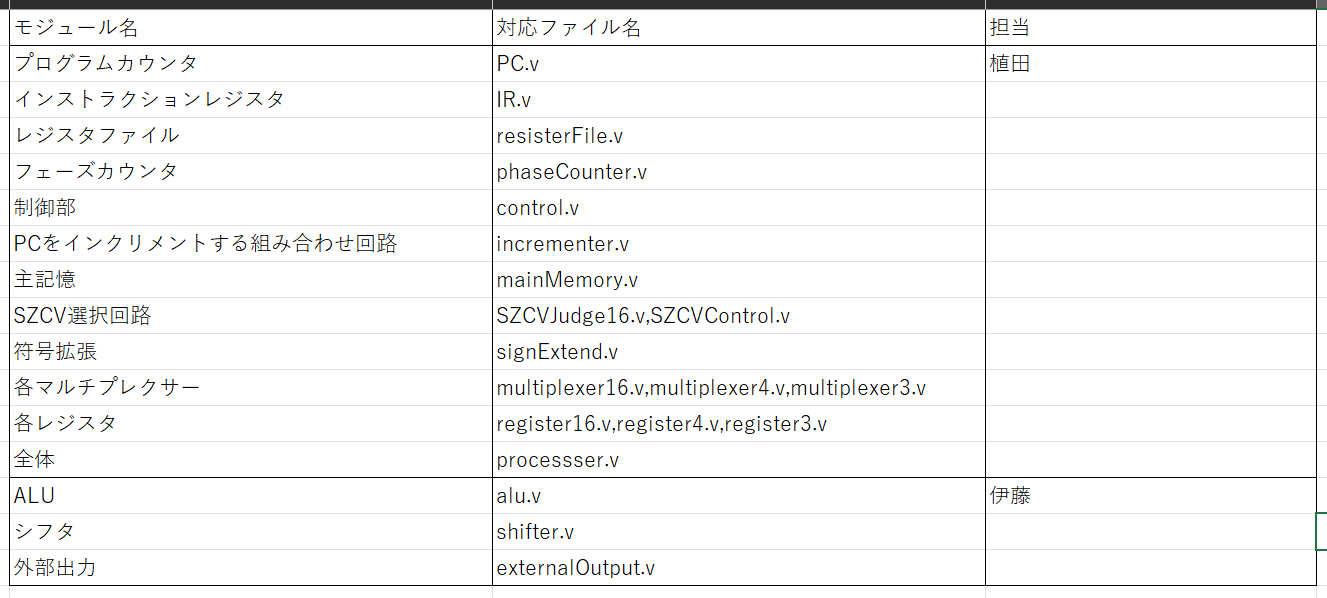
\includegraphics[scale = 0.43]{rolesDivision0506.png}
    \end{center}
    \caption{役割分担}
    \label{rolesDivision0422}
\end{figure}

\section{最終課題に対する現在の進捗状況}
授業資料の仕様を満たし、機能の拡張を行っていないsimplebプロセッサが完成した。
授業資料のsimple sampleの
Instruction TestとBubbleSortとFibonacciについて実機で実行したところ、
すべて正しく動作することが確認できた。
\section{今後の進捗計画}
今後、即値命令を追加する。また、パイプライン処理に必要な回路の構成を考え、
それらを実装していくつもりである。
パイプライン化に伴い、フェーズカウンタ、制御部などの仕様を大きく変える。


\end{document}